

\chapter{Sistema de deteção de intrusos}


No contexto desta dissertação houve necessidade de implementar um sistema de video-stream que permitisse detetar intrusos, maioritariamente pessoas ou animais de grande porte, que possam invadir as quintas onde se produz salicornia. Esta necessidade prende-se essencialmente com elevado custo do hardware do sistema de monitorização e também de eventuais instrumentos de elevado custo necessários ao cultivo desta espécie (e.g. geradores, maquinas elétricas para poda).

Neste capitulo será descrita a tecnologia de processamento de imagem utilizada tal como o algoritmo disponibilizado pela mesma. 


\section{Biblioteca de processamento de imagem: OpenCV}

O OpenCV, também conhecido por \textit{Open Source Computer Vision Library}, é uma biblioteca de software de visão por computador de código \textit{open source} (figura \ref{opencvlogo}). OpenCV foi construído para fornecer uma infra-estrutura comum para aplicações de visão computacional e para criar o uso da perceção da máquina nos produtos comerciais.

A biblioteca possui mais de 2500 algoritmos otimizados, que inclui um conjunto abrangente de algoritmos clássicos e avançados de visão computacional e algoritmos de \textit{machine learning}. Esses algoritmos podem ser usados para detectar e reconhecer rostos, identificar objetos, classificar ações humanas em vídeos, detetar movimentos numa câmara, seguir um objetos em movimento, produzir nuvens de pontos 3D de câmaras estéreo, entre outros.
OpenCV tem mais de 47 mil pessoas na comunidade de usuários e o número estimado de downloads superior a 7 milhões. A biblioteca é amplamente utilizada em empresas e grupos de pesquisa \cite{Itseez}.

O OpenCV é usado principalmente em aplicações de visão em tempo real. Esta biblioteca tem interfaces nas mais diversas linguagens: C++, C, Python, Java e MATLAB, embora seja nativamente escrito em C. OpenCV tem suporte para Windows, Linux e Mac OS\cite{Itseez}. 

\begin{figure}[!htb]
	\centering
	
\includegraphics[width=0.5\linewidth]{img/vision/opencv_logo.jpg}
	\caption{Logótipo OpenCV}
	\label{opencvlogo}
\end{figure}


\subsection{Conclusões}

Desde logo a escolha da tecnologia para processamento de imagem recaiu sobre o opencv não apenas por ser uma biblioteca bastante popular e possuir bastantes algoritmos implementados mas também por eu próprio possuir já algum background e projetos desenvolvidos neste neste contexto.


Pretendeu-se que este processamento fosse implementado em material já adquirido sem necessidade de gastos. Optou-se então por utilizar um \textit{Raspberry Pi} que juntamente com um \textit{Raspberry Pi camera module} (figura \ref{raspicam}) permitirá a aquisição de imagem e servirá também como \textit{controller module} ao sistema de aquisição de dados. 


\begin{figure}[!htb]
	\centering
	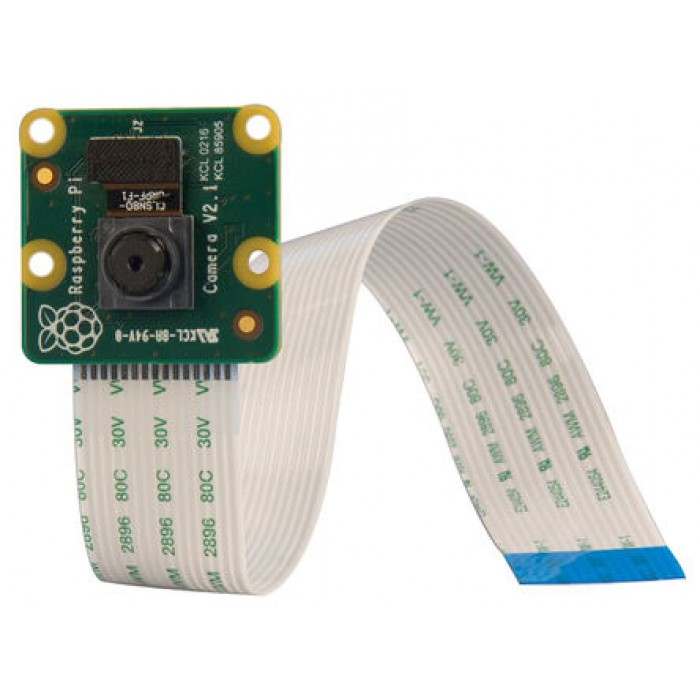
\includegraphics[width=0.3\linewidth]{img/hardware/camera_v2.jpg}
	\caption{Raspberry Pi Camera Board V2 8MP 1080p}
	\label{raspicam}
\end{figure}


Eis algumas das características principais do Raspberry Pi Camera Board V2:

\begin{itemize}
\item lente de foco fixo on-board
\item 150 milímetros CSI cabo da câmara incluída
\item 8 megapixels do sensor com capacidade de resolução nativa de 3.280 imagens estáticas de pixels x 2464
\item Suporta 1080p30, 720p60 e 640x480p90 vídeo
\item Tamanho 25 milímetros x 23 milímetros x 9 mm
\item Peso pouco mais de 3 g
\item Liga-se à placa de framboesa Pi por meio de um cabo de fita curta (fornecido)
\item Camera v2 é compatível com a última versão do Raspbian, sistema operacional preferido do Raspberry Pi
\end{itemize}


No que toca ao desenvolvimento, optou-se por utilizar o package picamera. Este pacote fornece  uma interface em Python (disponível para qualquer versão) para o módulo de câmara Raspberry Pi\footnote{http://picamera.readthedocs.io/en/release-1.13/}, permitindo uma fácil interação entre a aquisição da imagem e respetivo processamento. Neste contexto optou-se obviamente por utilizar a interface Python da biblioteca do OpenCV.



\section{Algoritmo de deteção de intrusos}
% artigo http://lear.inrialpes.fr/people/triggs/pubs/Dalal-cvpr05.pdf

De modo a estudar alguns algoritmos de deteção de pessoas foram estudados alguns artigos neste contexto. 


Para a resolução deste problema foi efetuados 


HOGDescriptor: classe que implementa um histograma de gradientes orientado ( [Dalal2005] ) detetor de objetos. 

hog = cv2.HOGDescriptor()
hog.setSVMDetector(cv2.HOGDescriptor\_getDefaultPeopleDetector())




Usado biblioteca do opencv que permite detectar 
HOGDescriptor


Deteção de intrusos: 

http://www.pyimagesearch.com/2015/11/09/pedestrian-detection-opencv/



versão simplificada: http://www.pyimagesearch.com/2015/02/16/faster-non-maximum-suppression-python/



Servidor em falsk 


deploy 
	https://iotbytes.wordpress.com/python-flask-web-application-on-raspberry-pi-with-nginx-and-uwsgi/



Dataset: %http://www.robots.ox.ac.uk/ActiveVision/Research/Projects/2009bbenfold_headpose/project.html


é usado um detector HOG juntamente com um classificador linear SVM 





parametros do método detectMultiScale do opencv 

\begin{itemize}
	\item \texttt{img}: parâmetro obrigatório. 
	\item \texttt{hitThreshold}: parâmetro opcional. 
	\item \texttt{winStride}: parâmetro opcional. 
	\item \texttt{padding}: parâmetro opcional.  Os valores típicos para preenchimento incluem  (8, 8) ,  (16, 16) ,  (24, 24) , e  (32, 32) .
	
		
	\item \texttt{scale}: parâmetro opcional. 
	\item \texttt{finalThreshold}: parâmetro opcional. 
	\item \texttt{useMeanShiftGrouping}: parâmetro opcional. 
\end{itemize}





Neste contexto apenas foram utilizados os seguintes parâmetros winStride, scale, padding. 



\section{Testes}

Foram considerados 4 frames de imagens .... e no apêndice X




\section{Implementação}


\subsection{Flask}

Flask é considerada uma microframework web desenvolvida em Python e baseado nas bibliotecas WSGI Werkzeug e Jinja2. Escolhi esta microframework pois pretende-se que esta seja executada num microcontrolador com baixos recursos. Para além disso, considera-se ser de fácil aprendizagem relativamente ao Django (já abordado na capitulo XX) e com uma ótima documentação. 




\subsection{Servidor web NGNIX}

\section{Considerações finais}

